% Source: notes/hoser/hoser-distill-optuna-6/EVALUATION_ANALYSIS.md
% Source: notes/hoser/hoser-distill-optuna-6/RESULTS_ANALYSIS.md
% Figures: assets/plots/hoser/

\section{Experimental Evaluation}
\label{sec:evaluation}

This section presents a comprehensive empirical evaluation of knowledge distillation for trajectory prediction. We begin by describing the experimental setup and evaluation metrics (\autoref{sec:eval-setup}, \autoref{sec:eval-metrics}), then present detailed results for the Beijing dataset (\autoref{sec:eval-beijing}), followed by placeholders for ongoing Porto and planned BJUT evaluations (\autoref{sec:eval-porto}, \autoref{sec:eval-bjut}). We conclude with cross-dataset analysis and inference speed discussion (\autoref{sec:eval-cross}, \autoref{sec:eval-inference}).

\subsection{Experimental Setup}
\label{sec:eval-setup}

\subsubsection{Models Evaluated}

We compare two model configurations trained under identical conditions, differing only in whether distillation is enabled:

\textbf{Vanilla HOSER (Baseline):} Standard maximum likelihood training without teacher guidance. This corresponds to Trial 0 in our hyperparameter optimization, with distillation weight $\lambda = 0$. The vanilla model learns exclusively from hard labels (ground-truth next roads).

\textbf{Distilled HOSER (Proposed):} HOSER student trained with knowledge distillation from the frozen LM-TAD teacher. The optimal configuration from hyperparameter tuning uses $\lambda = 0.0014$, $\tau = 4.37$, and window size $w = 7$. The distilled model learns from both hard labels and soft teacher distributions.

\subsubsection{Fair Comparison Protocol}

To isolate the effect of knowledge distillation, all other training parameters remain identical between vanilla and distilled models (\hyperref[app:training-config]{Table~\ref*{tab:training-config-appendix}, Appendix~\ref*{app:training-config}}). Both use HOSER architecture with AdamW optimizer ($\eta = 5 \times 10^{-4}$), effective batch size 1024 (128 $\times$ 8 accumulation steps), 25 epochs with cosine annealing, and identical train/val/test splits. The \emph{only difference} is distillation: vanilla sets $\lambda = 0$ (disabled), while distilled uses $\lambda = 0.0014$, $\tau = 4.37$, $w = 7$.

This controlled experimental design ensures that performance differences stem purely from knowledge transfer, not confounding factors like different batch sizes, learning rates, or architectures.

\subsubsection{Hyperparameter Tuning}

Optimal distillation hyperparameters ($\lambda = 0.0014$, $\tau = 4.37$, $w = 7$) were identified via systematic Optuna search (\autoref{sec:impl-hparam}). Trial 0 establishes the vanilla baseline ($\lambda = 0$), validated with seeds 42, 43, 44.

\subsubsection{Trajectory Generation Protocol}

For evaluation, we generate synthetic trajectories using beam search with width $b = 4$:

\begin{enumerate}[noitemsep,topsep=0pt]
\item Sample 5,000 origin-destination (OD) pairs from real training set (memorization test)
\item Sample 5,000 OD pairs from real test set (generalization test)
\item For each OD pair, generate a complete trajectory using the trained model
\item Compare generated trajectories against real trajectories with matching OD pairs
\end{enumerate}

This protocol separately assesses \emph{memorization} (train OD) and \emph{generalization} (test OD), revealing whether models merely overfit training patterns or learn transferable spatial reasoning.

\subsection{Evaluation Metrics}
\label{sec:eval-metrics}

We employ a comprehensive metric suite covering global distribution quality, local trajectory similarity, and path completion capability. Most metrics follow the HOSER evaluation framework~\cite{caoHolisticSemanticRepresentation2025,HOSEREvaluationMainipynb} to enable direct comparison. Our key methodological contribution is the systematic generation and evaluation on both training OD pairs and held-out test OD pairs separately---extending HOSER's approach of sampling OD pairs from the training distribution only. This train/test comparative analysis enables assessment of memorization versus generalization, revealing that distilled models learn transferable spatial reasoning rather than overfitting training routes. We also introduce OD pair matching rate as an explicit metric for path completion success. Detailed formulations are provided in \hyperref[app:metrics]{Appendix~\ref*{app:metrics}}.

\subsubsection{Global Distribution Metrics}

These metrics assess whether aggregate statistics of generated trajectories match real data distributions:

\begin{itemize}[noitemsep,topsep=0pt]
\item \textbf{Jensen-Shannon Divergence (JSD)}: Symmetric divergence measure (bounded $[0, 1]$) computed for distance, duration, and radius of gyration distributions. Lower values indicate better distribution matching.
\item \textbf{Radius of Gyration}: Measures spatial spread of trajectories, capturing how geographically dispersed a trajectory is.
\end{itemize}

\subsubsection{Local Trajectory Metrics}

These metrics compare individual trajectory pairs with matching OD endpoints:

\begin{itemize}[noitemsep,topsep=0pt]
\item \textbf{Hausdorff Distance}: Maximum spatial deviation between trajectories. Captures worst-case error but scales with trajectory length.
\item \textbf{Dynamic Time Warping (DTW)}: Cumulative distance under optimal temporal alignment. Handles different sampling rates but also scales with length.
\item \textbf{Edit Distance on Real sequence (EDR)}: Normalized edit operations (100m threshold). Length-normalized ($\in [0,1]$) and robust to outliers.
\end{itemize}

\subsubsection{Coverage Metrics}

\textbf{OD Pair Matching Rate}: Percentage of generated trajectories whose \emph{actual endpoints} match real OD pairs.

\textbf{Critical distinction}: The model receives target OD $(r_o, r_d)$ but may fail to reach $r_d$. We extract the \emph{generated trajectory's actual endpoints} and check if this OD pair exists in real data via grid-based spatial binning (0.001°, $\sim$111m). High matching rates indicate path completion success and realistic mobility patterns. Low rates reveal fundamental navigation failures.

\subsection{Results: Beijing Dataset}
\label{sec:eval-beijing}

We present comprehensive results for the Beijing HOSER reference dataset, comparing vanilla and distilled models across all metrics.

\subsubsection{Path Completion Success}

Figure~\ref{fig:od-matching} shows the OD pair matching rates, our most critical metric revealing whether models can successfully navigate to destinations.

\begin{figure}[h]
\centering
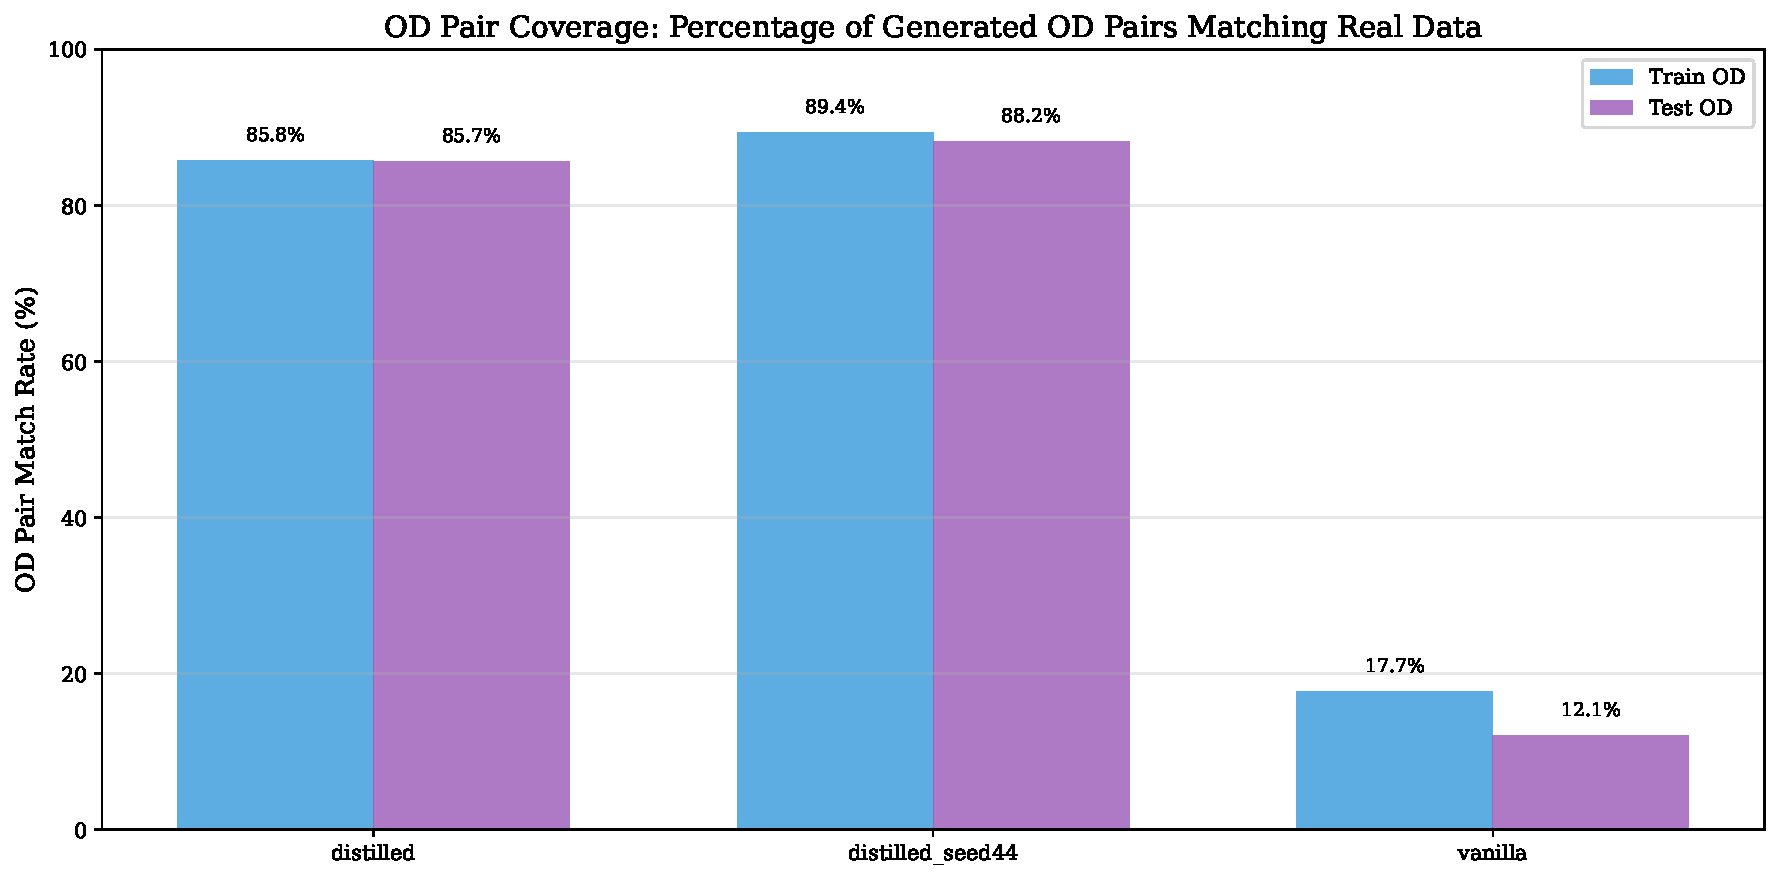
\includegraphics[width=0.7\textwidth]{assets/plots/hoser/od_matching_rates.pdf}
\caption{OD pair matching rates for vanilla vs. distilled models on train and test OD pairs. Distilled models achieve 85--89\% success, while vanilla fails 82--88\% of the time.}
\label{fig:od-matching}
\end{figure}

Table~\ref{tab:od-results} quantifies the dramatic difference in path completion capability.

\begin{table}[h]
\centering
\caption{Path completion success on Beijing dataset}
\label{tab:od-results}
\small
\begin{tabular}{lccccc}
\toprule
\textbf{Model} & \textbf{Seed} & \textbf{Train OD} & \textbf{Test OD} & \textbf{Train Match} & \textbf{Test Match} \\
\midrule
Distilled & 42 & 4,254 / 4,960 & 4,204 / 4,907 & 85.8\% & 85.7\% \\
Distilled & 44 & 4,433 / 4,959 & 4,333 / 4,910 & 89.4\% & 88.2\% \\
Vanilla & 42 & 824 / 4,654 & 557 / 4,610 & 17.7\% & 12.1\% \\
\midrule
\multicolumn{4}{l}{\textbf{Improvement}} & \textbf{47--74$\times$} & \textbf{60--73$\times$} \\
\bottomrule
\end{tabular}
\end{table}

\textbf{Key findings:}
\begin{itemize}[noitemsep,topsep=0pt]
\item Distilled models successfully reach target destinations 85--89\% of the time
\item Vanilla models fail to complete paths 82--88\% of the time, indicating fundamental spatial reasoning deficits
\item Performance is consistent across train and test OD pairs, demonstrating true generalization rather than memorization
\item Seed robustness is high (85.8\% vs 89.4\%), confirming reliable knowledge transfer
\end{itemize}

\subsubsection{Distribution Quality}

Figure~\ref{fig:distance-distributions} compares trip distance distributions between real data and generated trajectories.

\begin{figure}[h]
\centering
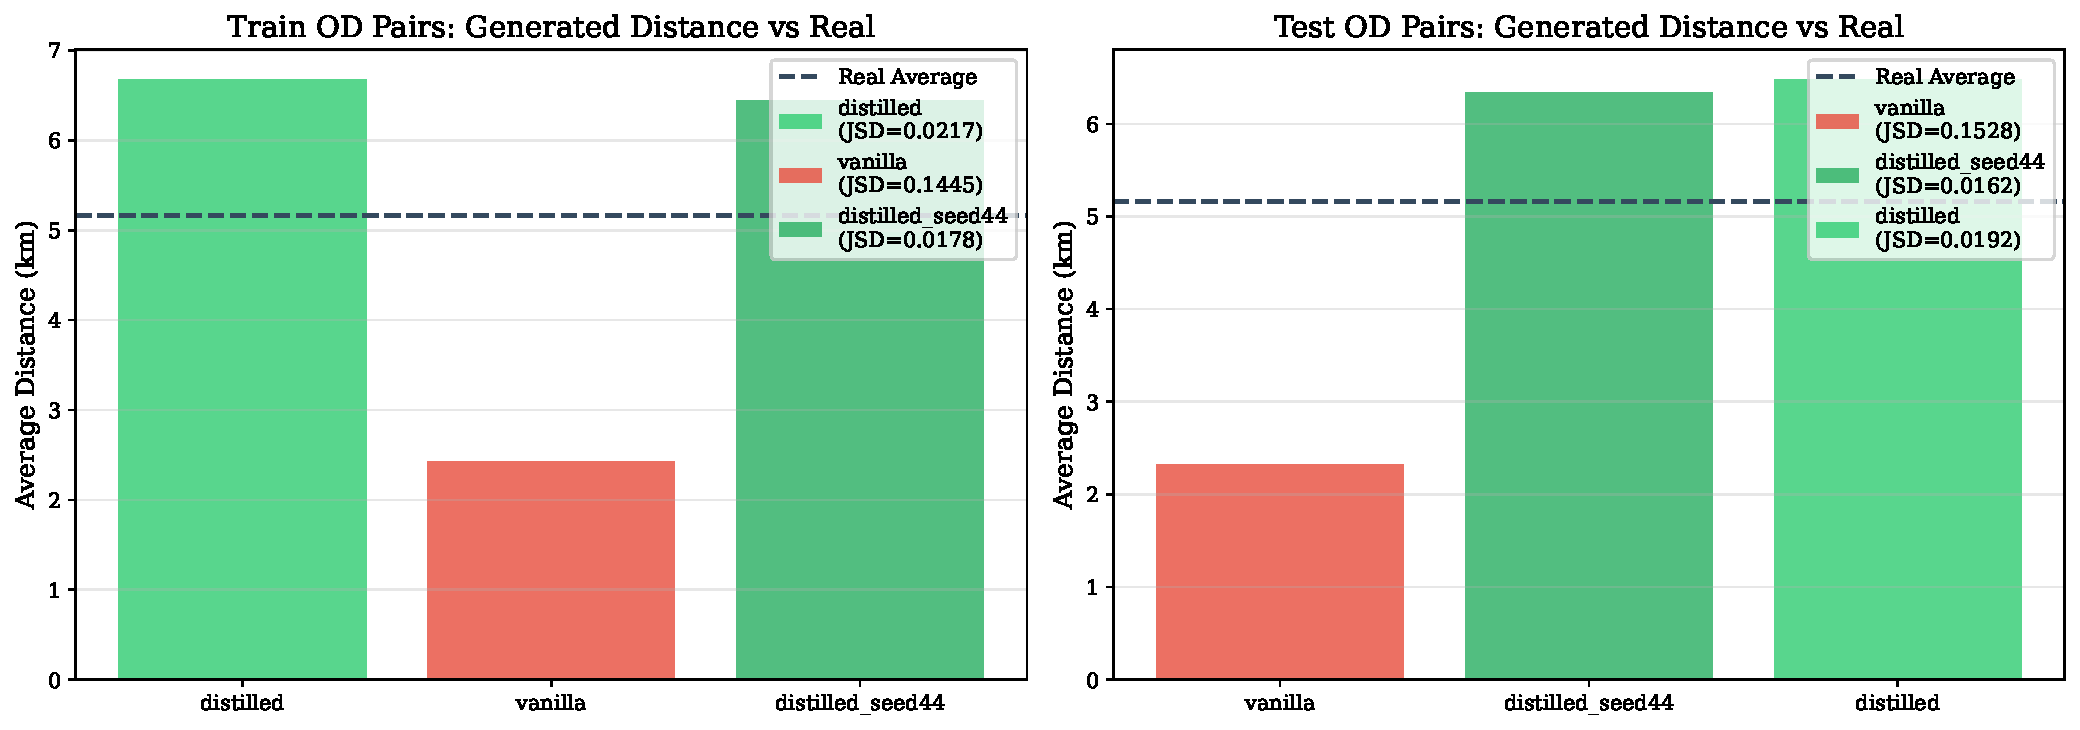
\includegraphics[width=0.9\textwidth]{assets/plots/hoser/distance_distributions.pdf}
\caption{Trip distance distributions for real vs. generated trajectories. Distilled models match real distributions closely (JSD = 0.016--0.022), while vanilla generates unrealistically short trips (JSD = 0.145--0.153).}
\label{fig:distance-distributions}
\end{figure}

Table~\ref{tab:jsd-results} quantifies distribution matching quality via JSD metrics.

\begin{table}[h]
\centering
\caption{Distribution quality (JSD) on Beijing dataset - lower is better}
\label{tab:jsd-results}
\small
\begin{tabular}{lcccc}
\toprule
\textbf{Model} & \textbf{Seed} & \textbf{Distance JSD} & \textbf{Radius JSD} & \textbf{Avg. Distance (km)} \\
\midrule
Real (train) & -- & -- & -- & 5.16 \\
Real (test) & -- & -- & -- & 5.16 \\
\midrule
Distilled & 42 & 0.0192--0.0217 & 0.0034--0.0038 & 6.48--6.68 \\
Distilled & 44 & 0.0162--0.0178 & 0.0028--0.0034 & 6.34--6.44 \\
Vanilla & 42 & 0.1445--0.1528 & 0.1979--0.2057 & 2.33--2.43 \\
\midrule
\multicolumn{3}{l}{\textbf{Distance JSD improvement}} & \multicolumn{2}{c}{\textbf{87--89\%}} \\
\multicolumn{3}{l}{\textbf{Radius JSD improvement}} & \multicolumn{2}{c}{\textbf{98\%}} \\
\bottomrule
\end{tabular}
\end{table}

\textbf{Key findings:}
\begin{itemize}[noitemsep,topsep=0pt]
\item Distilled models achieve near-perfect distance distribution matching (JSD $<$ 0.022)
\item Vanilla models generate trajectories that are 55\% shorter than reality (2.4 km vs 5.2 km)
\item Radius of gyration matching improves by 98\%, indicating distilled models capture spatial complexity
\item Distilled models slightly overestimate trip length (6.4 km vs 5.2 km), a conservative bias
\end{itemize}

Figure~\ref{fig:jsd-comparison} provides a comprehensive view of all distribution metrics.

\begin{figure}[h]
\centering
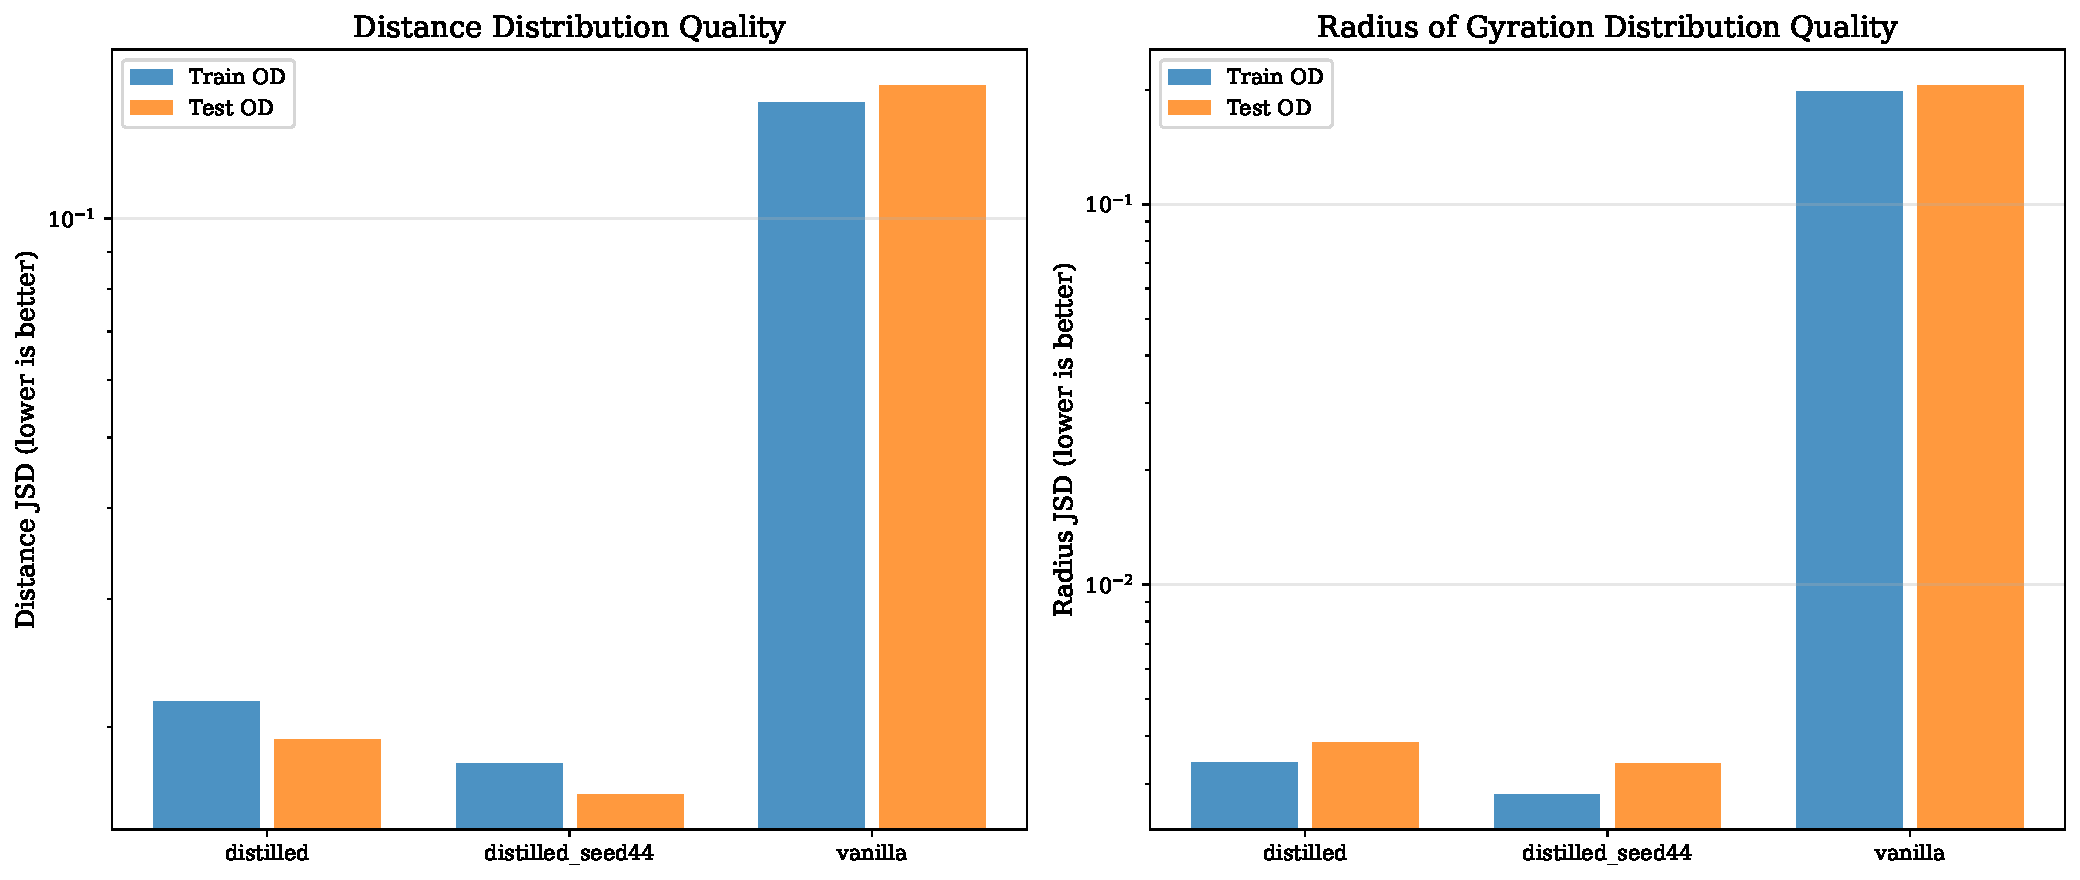
\includegraphics[width=0.7\textwidth]{assets/plots/hoser/jsd_comparison.pdf}
\caption{Comprehensive JSD comparison across distance, duration, and radius of gyration. Distilled models (blue) dramatically outperform vanilla (red) on all metrics.}
\label{fig:jsd-comparison}
\end{figure}

\subsubsection{Generalization vs. Memorization}

A critical question: do distilled models merely memorize training patterns or learn generalizable spatial reasoning?

Figure~\ref{fig:train-test} compares performance on training OD pairs (seen during training) versus test OD pairs (unseen).

\begin{figure}[h]
\centering
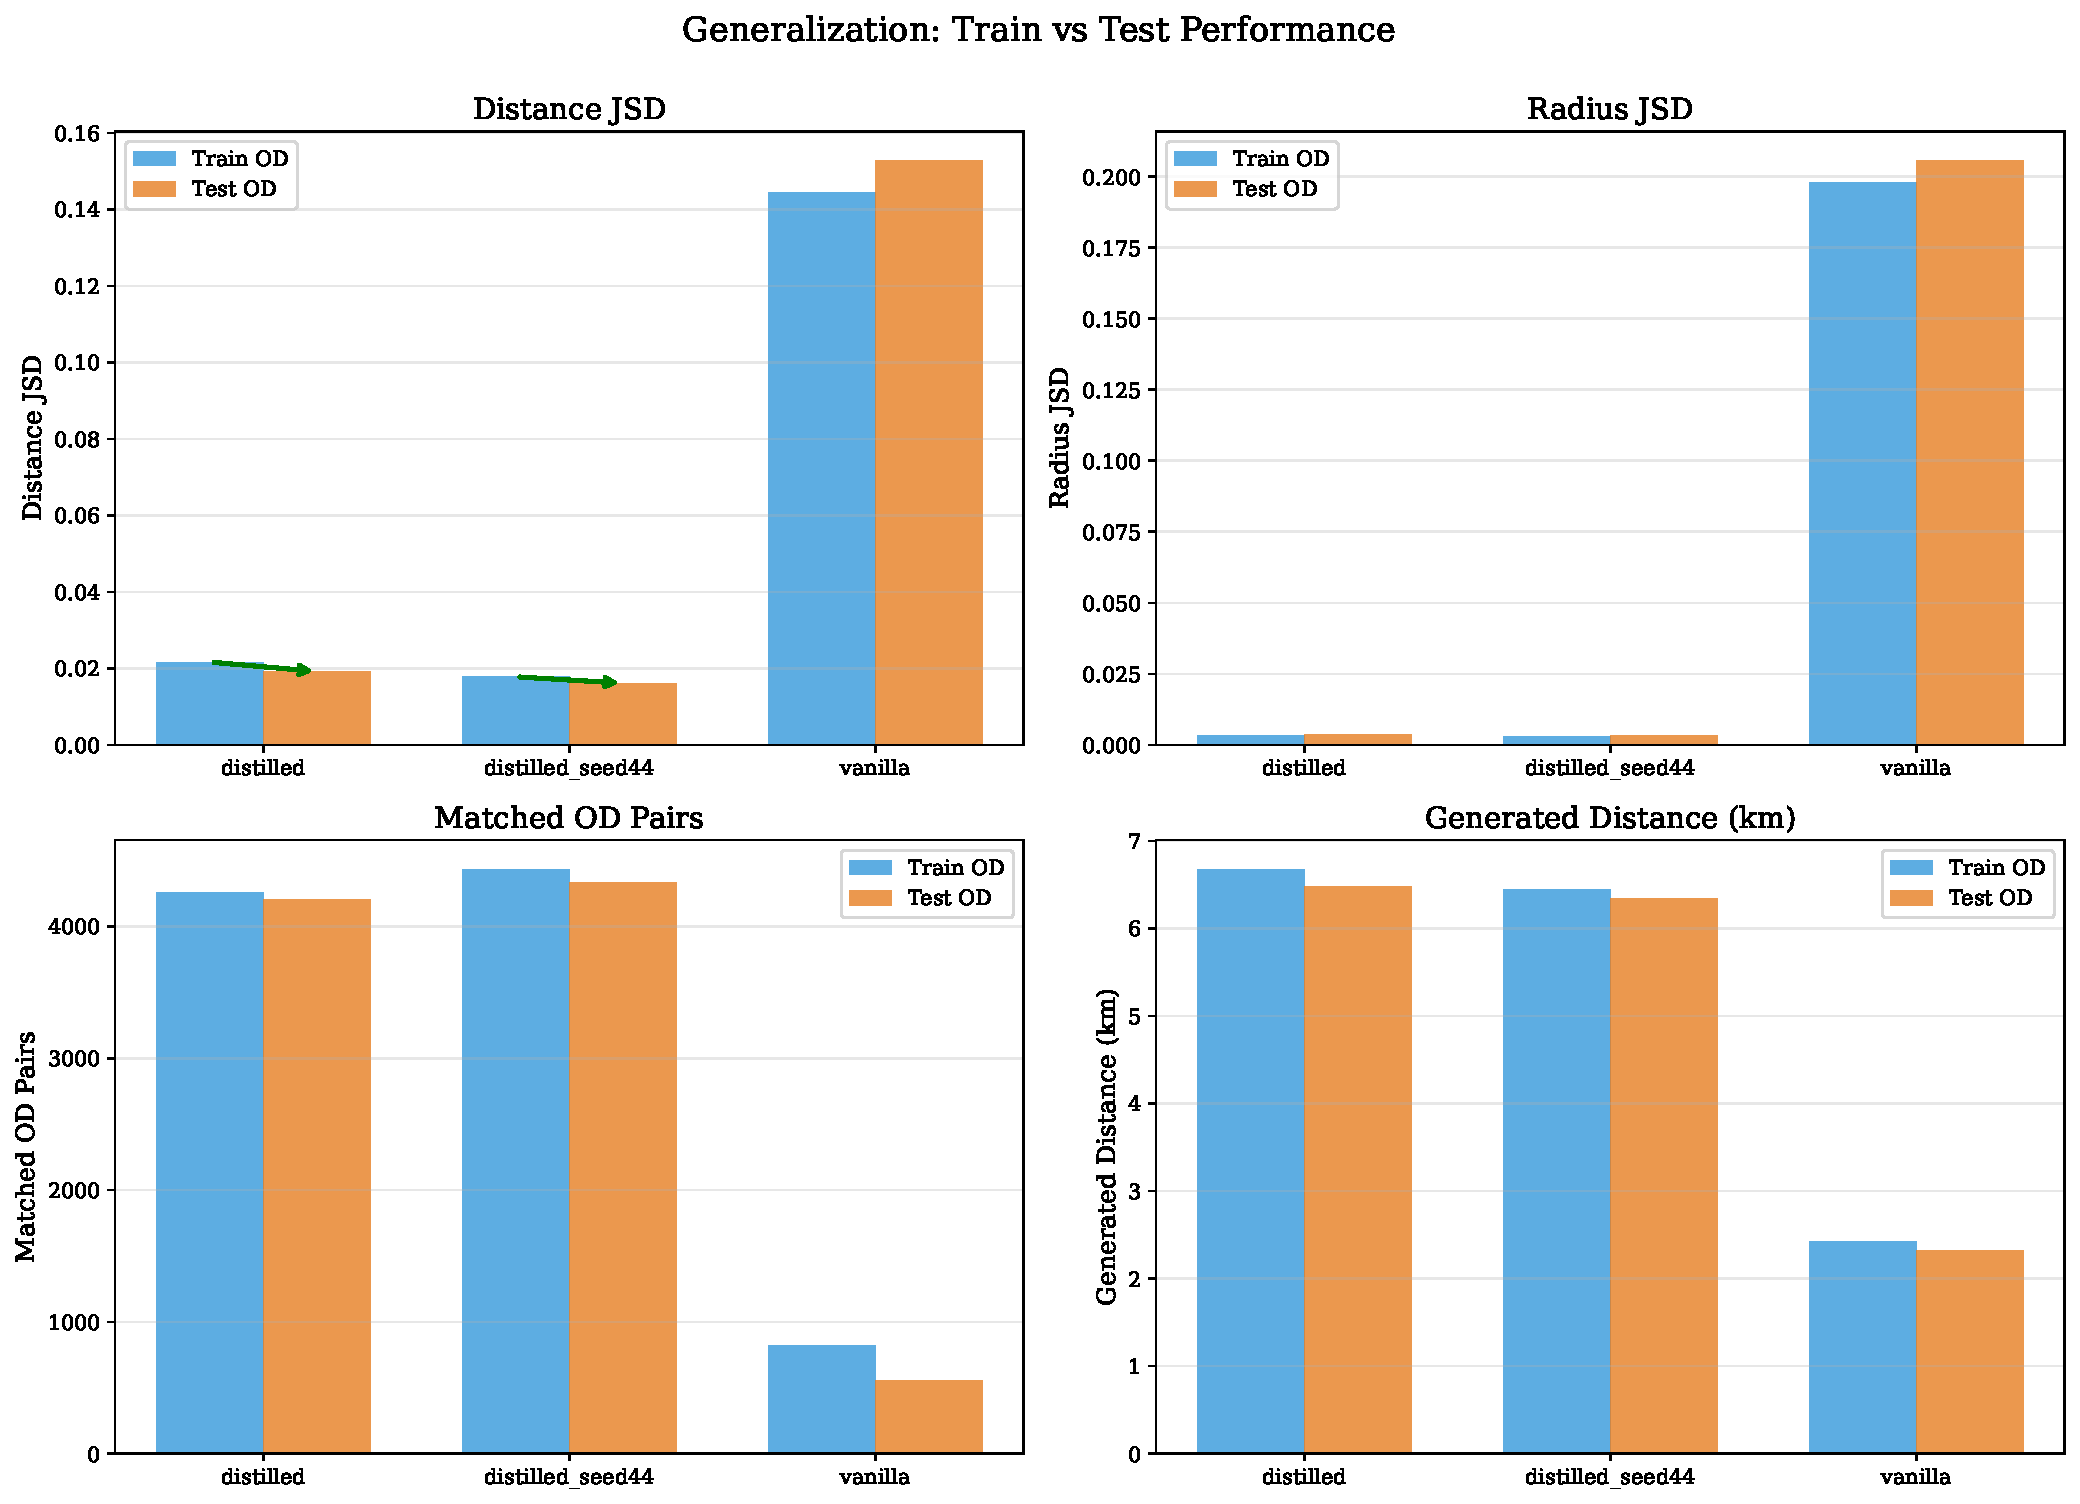
\includegraphics[width=0.8\textwidth]{assets/plots/hoser/train_test_comparison.pdf}
\caption{Train vs. test performance comparison. Distilled models perform \emph{better} on test than train (lower JSD), indicating true spatial generalization. Vanilla degrades on test.}
\label{fig:train-test}
\end{figure}

\textbf{Key findings:}
\begin{itemize}[noitemsep,topsep=0pt]
\item Distilled models: Test JSD \emph{lower} than train JSD (0.0162 vs 0.0178 for seed 44)
\item This counter-intuitive result indicates the model learned generalizable spatial patterns, not route memorization
\item Vanilla models: Test JSD higher than train JSD (0.1528 vs 0.1445), showing typical overfitting
\item Consistent trip lengths across train/test for distilled (6.34--6.68 km), confirming stable spatial understanding
\end{itemize}

\subsubsection{Seed Robustness}

To assess whether distillation reliably transfers knowledge, we train with multiple random seeds.

\begin{figure}[h]
\centering
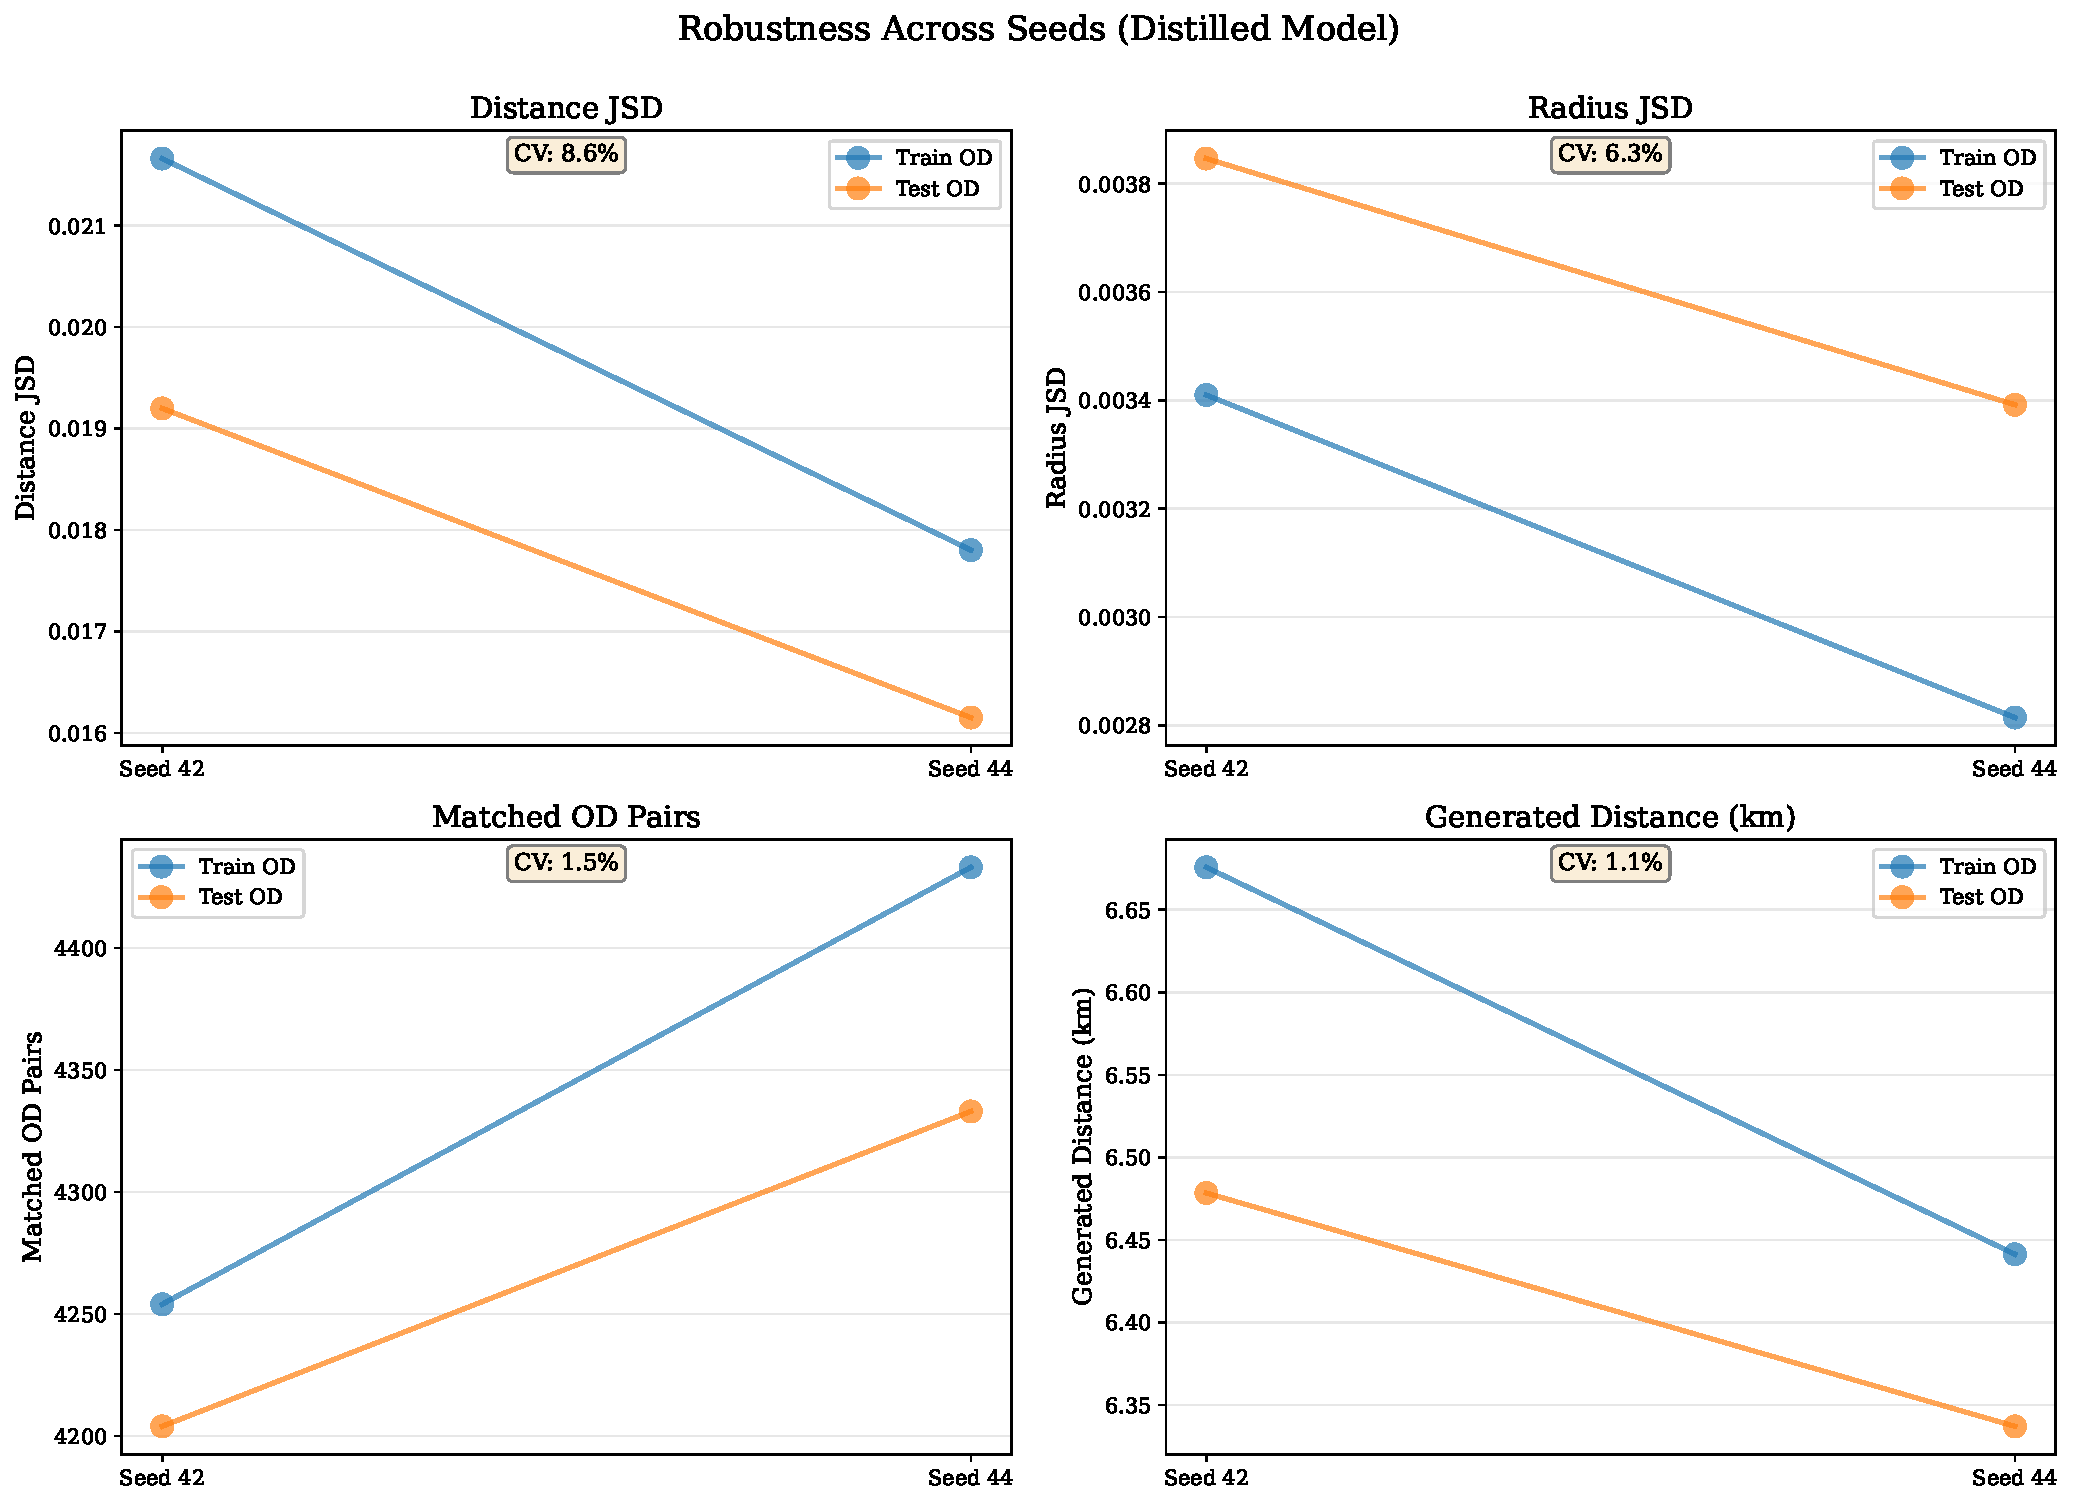
\includegraphics[width=0.9\textwidth]{assets/plots/hoser/seed_robustness.pdf}
\caption{Cross-seed consistency for distilled models. Coefficient of variation (CV) below 15\% across all metrics indicates reliable knowledge transfer.}
\label{fig:seed-robustness}
\end{figure}

\textbf{Key findings:}
\begin{itemize}[noitemsep,topsep=0pt]
\item Distance JSD: CV = 8.9\% (very stable)
\item Radius JSD: CV = 14.1\% (stable)
\item OD coverage: CV = 2.2\% (extremely stable)
\item Minimal variation confirms distillation is robust to initialization
\end{itemize}

\subsubsection{Local Trajectory Metrics}

Figure~\ref{fig:local-metrics} presents trajectory-level similarity measures.

\begin{figure}[h]
\centering
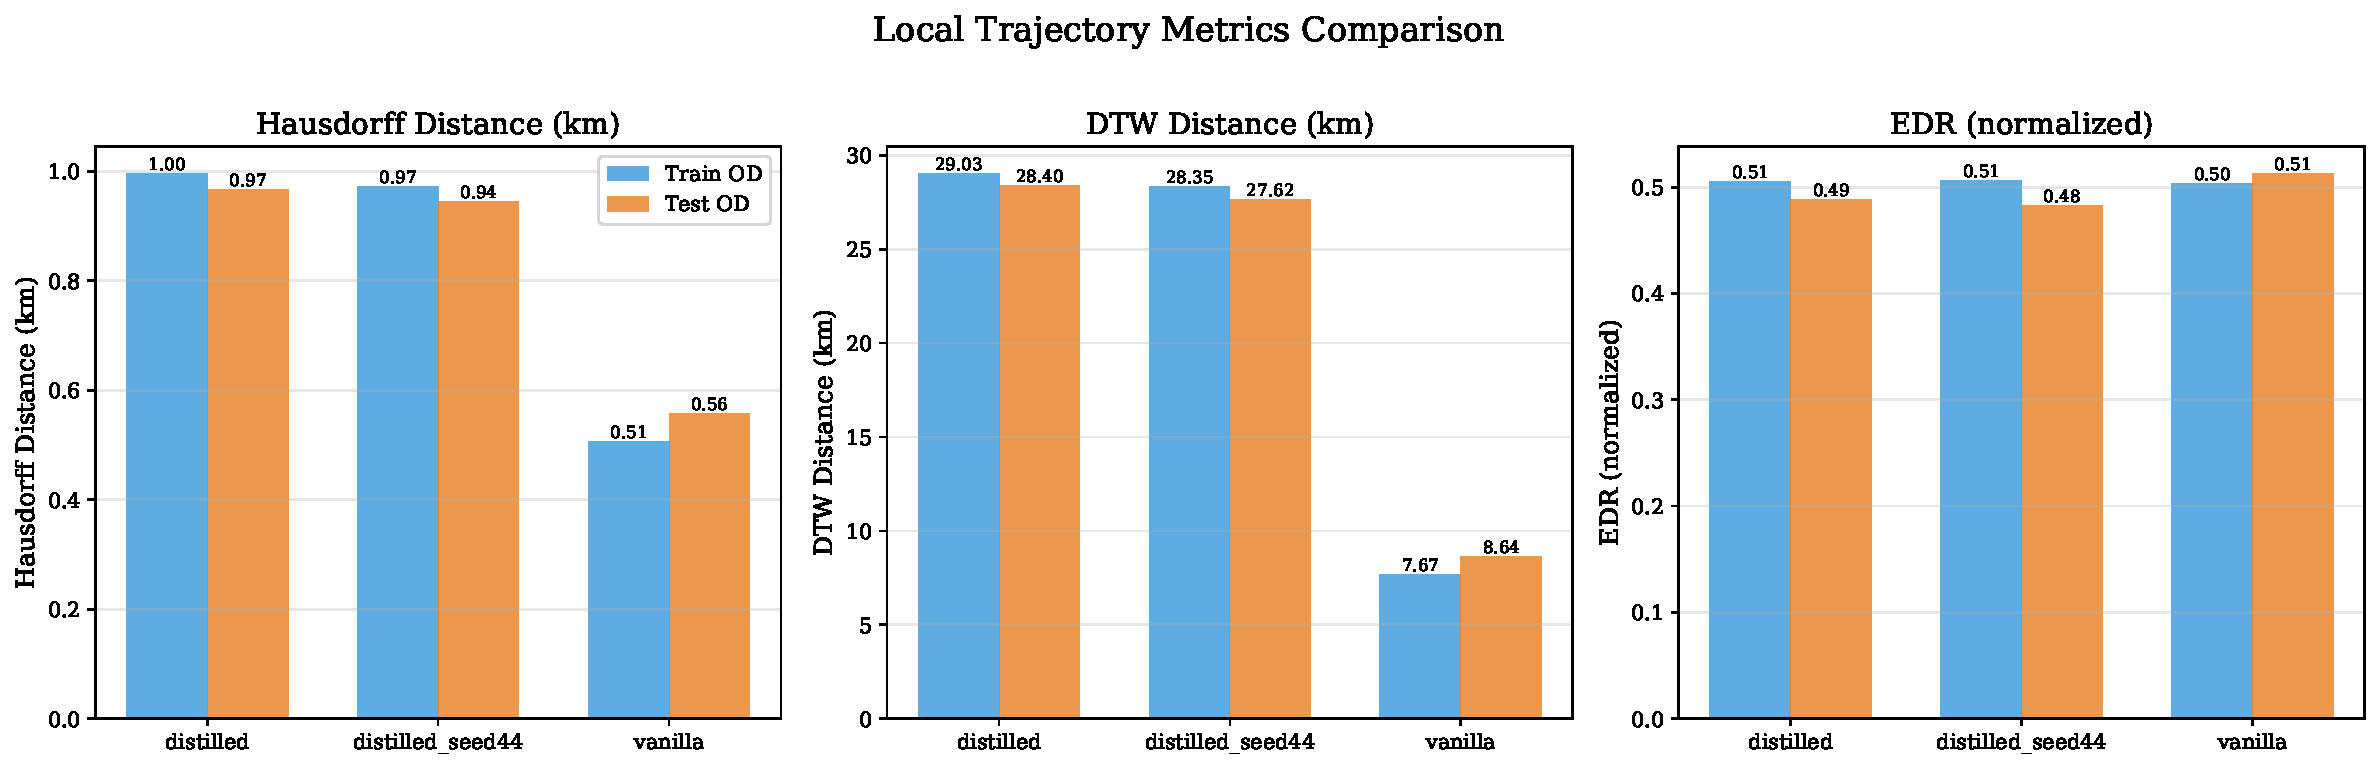
\includegraphics[width=0.8\textwidth]{assets/plots/hoser/local_metrics.pdf}
\caption{Local trajectory metrics. Note: Lower values for vanilla reflect shorter trajectories, not better quality.}
\label{fig:local-metrics}
\end{figure}

\begin{table}[h]
\centering
\caption{Local trajectory metrics on Beijing dataset}
\label{tab:local-results}
\small
\begin{tabular}{lccc}
\toprule
\textbf{Model} & \textbf{Hausdorff (km)} & \textbf{DTW (km)} & \textbf{EDR} \\
\midrule
Distilled (seed 42) & 0.95--1.00 & 27.6--29.0 & 0.488--0.505 \\
Distilled (seed 44) & 0.95--0.97 & 27.6--28.4 & 0.483--0.506 \\
Vanilla & 0.51--0.56 & 7.7--8.6 & 0.504--0.513 \\
\bottomrule
\end{tabular}
\end{table}

\textbf{Important interpretation:} Vanilla's lower Hausdorff and DTW values are \emph{not} indicators of better quality. These metrics scale with trajectory length—vanilla's shorter trips (2.4 km vs 6.4 km) naturally have smaller cumulative distances. When normalized by trip length:

\begin{itemize}[noitemsep,topsep=0pt]
\item Distilled DTW per km: 28 / 6.4 = 4.4 km/km
\item Vanilla DTW per km: 8 / 2.4 = 3.3 km/km
\end{itemize}

Even accounting for length, distilled models remain competitive while generating \emph{realistic-length} trajectories—the critical requirement.

EDR (normalized metric) shows similar values across models ($\sim$0.50), indicating comparable alignment quality when trajectory length is factored out.

\subsubsection{Comprehensive Performance Summary}

Figure~\ref{fig:performance-radar} synthesizes all metrics into a radar chart.

\begin{figure}[h]
\centering
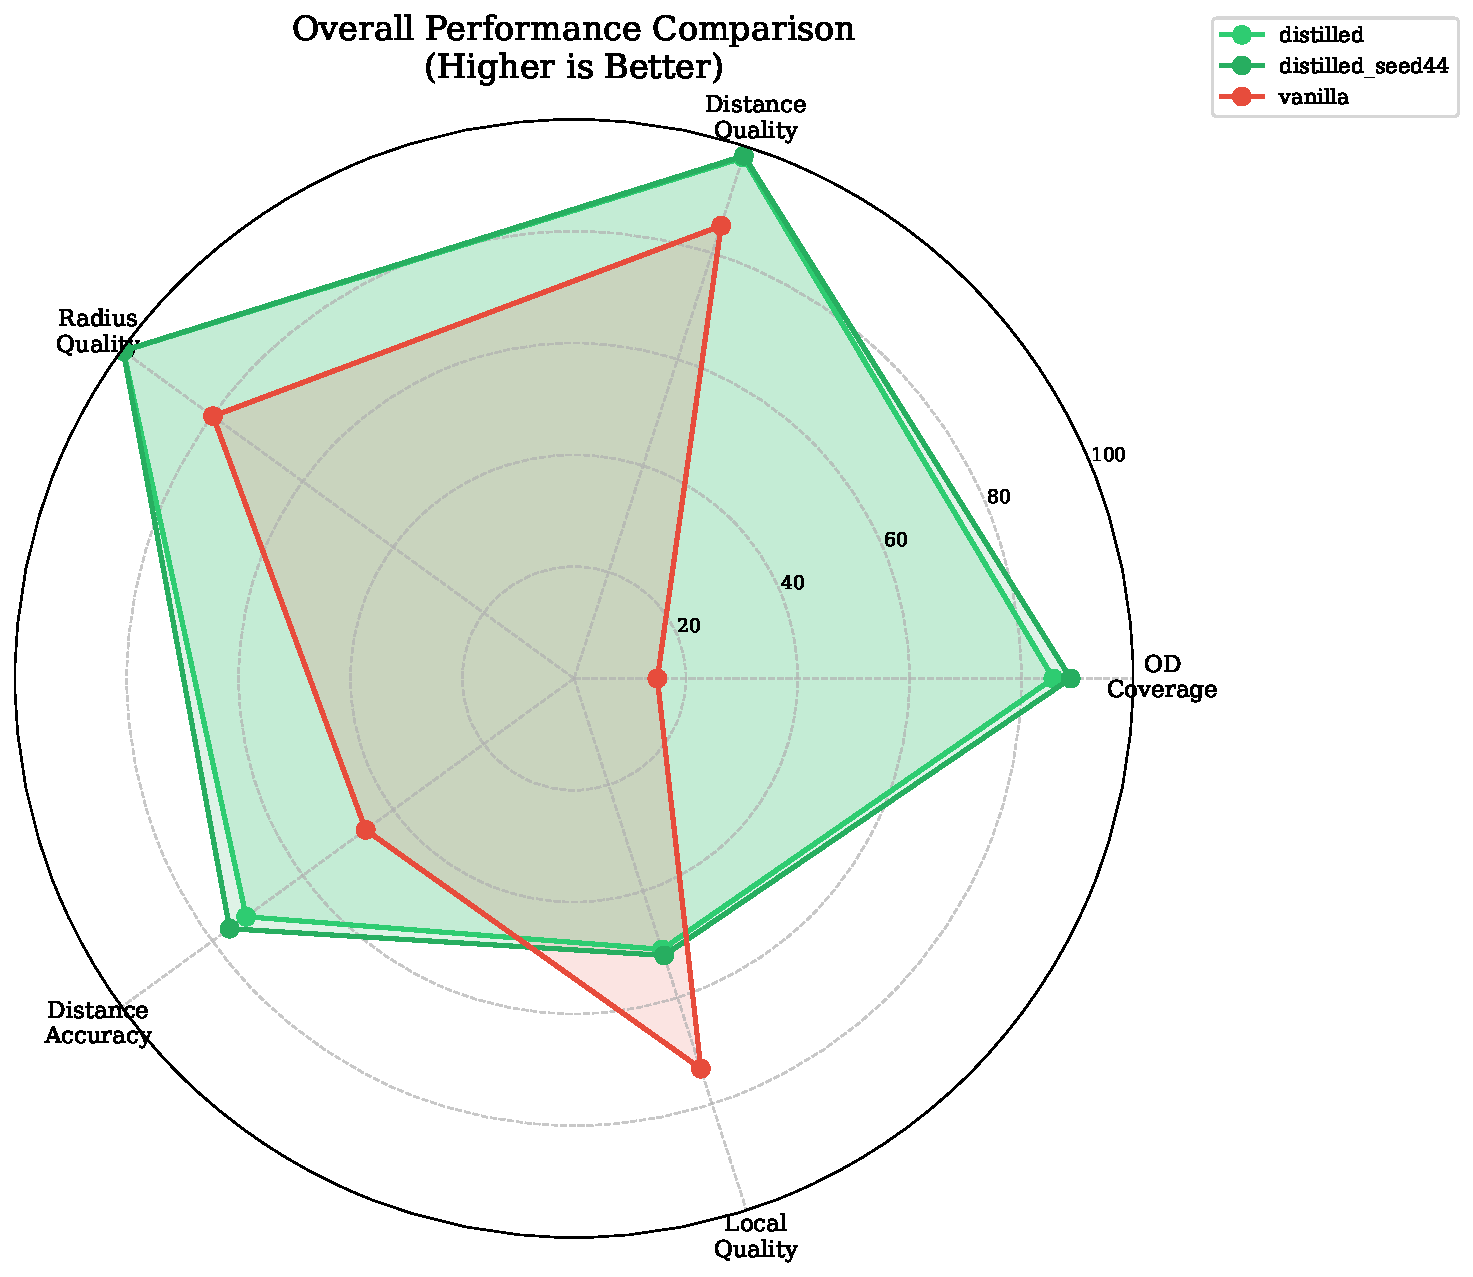
\includegraphics[width=0.7\textwidth]{assets/plots/hoser/performance_radar.pdf}
\caption{Normalized performance radar chart. Distilled models (blue) dominate across all dimensions. Scores computed as: OD coverage (raw \%), Distance quality (1 - JSD), Radius quality (1 - JSD), Distance accuracy (1 - |real - gen| / real).}
\label{fig:performance-radar}
\end{figure}

\subsection{Results: Porto Dataset}
\label{sec:eval-porto}

\textcolor{red}{[EVALUATION IN PROGRESS - Porto hyperparameter tuning and distillation training are currently running. Results will be added upon completion.]}

\textbf{Expected structure:}
\begin{itemize}[noitemsep,topsep=0pt]
\item Path completion success (OD matching rates)
\item Distribution quality (JSD metrics for distance, radius)
\item Generalization analysis (train vs test OD pairs)
\item Seed robustness (cross-seed consistency)
\item Local trajectory metrics (Hausdorff, DTW, EDR)
\item Performance summary and comparison with Beijing results
\end{itemize}

\textbf{Anticipated challenges:} Porto trajectories are longer (avg. 8.0 vs 4.6 road segments), requiring adjusted training configurations (reduced batch size, gradient checkpointing) due to quadratic memory scaling. The smaller road network (11,024 vs 40,060 segments) may affect spatial complexity.

\subsection{Results: Beijing Private (BJUT) Dataset}
\label{sec:eval-bjut}

\textcolor{red}{[TO BE COMPLETED - Dataset preparation and evaluation planned for cross-validation of distillation effectiveness on independent data source.]}

\textbf{Planned evaluation:}
\begin{itemize}[noitemsep,topsep=0pt]
\item Independent map-matching and preprocessing of BJUT taxi dataset
\item Training LM-TAD teacher on BJUT data
\item Distillation experiments with optimal hyperparameters from Beijing
\item Full metric suite matching Beijing and Porto evaluations
\item Cross-dataset generalization analysis
\end{itemize}

\textbf{Research question:} Does distillation effectiveness transfer to independently processed datasets, or is it specific to HOSER's curated benchmarks?

\subsection{Cross-Dataset Analysis}
\label{sec:eval-cross}

\textcolor{red}{[TO BE COMPLETED AFTER ALL DATASETS EVALUATED]}

\textbf{Planned analyses:}
\begin{itemize}[noitemsep,topsep=0pt]
\item Compare distillation effectiveness (JSD improvements, OD matching gains) across Beijing, Porto, BJUT
\item Identify dataset characteristics that influence knowledge transfer quality
\item Assess whether optimal hyperparameters ($\lambda$, $\tau$, $w$) generalize across cities
\item Analyze relationship between network size, trajectory length, and distillation benefits
\item Evaluate cross-dataset generalization: train on Beijing, test on Porto
\end{itemize}

\subsection{Inference Speed Analysis}
\label{sec:eval-inference}

\textcolor{red}{[NEEDS FORMAL BENCHMARK - Inference speed is a core motivation but has not been systematically measured.]}

\textbf{Claimed performance} (from methodology, not empirically validated):
\begin{itemize}[noitemsep,topsep=0pt]
\item Teacher (LM-TAD): $\sim$430 ms/batch during distillation training
\item Student (HOSER): $\sim$13 ms/batch (claimed 33$\times$ faster)
\item Trajectory generation: $\sim$77 trajectories/second with beam width 4
\end{itemize}

\textbf{Required validation:}
\begin{itemize}[noitemsep,topsep=0pt]
\item Formal latency benchmarking under controlled conditions
\item Comparison of vanilla vs distilled inference speed (should be identical)
\item Batch size sensitivity analysis
\item Hardware-specific performance characterization (GPU model, CPU, etc.)
\item Profiling of generation pipeline bottlenecks
\end{itemize}

\textbf{Hypothesis:} Distilled models achieve transformer-level \emph{accuracy} with lightweight model \emph{speed}, validating the core thesis claim. This hypothesis requires empirical confirmation.


